\documentclass[a4paper, 11pt, french, oneside]{book}
\usepackage[utf8]{inputenc}
\usepackage[T1]{fontenc}
\usepackage[francais]{babel}
\usepackage{graphicx}
\usepackage{charter}
\usepackage{color}
\usepackage{multirow}
\usepackage{parskip}
		
\begin{document}
	\begin{titlepage}
		\begin{center}
			
\includegraphics[width=12cm]{linux.jpg}%
			\hspace{60pt}%
			\vspace{50pt}%
			\LARGE
			\textbf{Résumé du cours de Linux en Latex}\\
			\color{red}
			\textbf{Classe X81}\\
			Ambroise - Anouar - Quentin\\
			\vspace{50pt}%
			
\includegraphics[width=8cm]{latex.jpg}%
		\end{center}
	\end{titlepage}
		      
	\tableofcontents
	\frontmatter
	\mainmatter
	\chapter{Les outils essentiels}
		\section{Les 7 premières commandes}
         %\begin{flushleft}
         • \textbf {\textit{\color{red}whoaim}} : Renvoie votre login-name actuel.\\
         • \textbf {\textit{\color{red}hostname}} : Renvoie le nom de la machine sur laquelle vous travaillez.\\
         • \textbf {\textit{\color{red}date}} : Renvoie la date actuelle.\\
         • \textbf {\textit{\color{red}uname}} : Renvoie des informations sur le système actuel.\\
         • \textbf{\textit{\color{red}passwd}} : Permet au user de changer son mot-de-passe et permet à l’administrateur ou le root de changer le mot-de-passe d’un user.\\
         • \textbf{\textit{\color{red}touch}} : Permet la création d’un fichier vide ou la mise à jour de la date de modification d’un ficher existant.\\
         • \textbf{\textit{\color{red}last}} : Renvoie la liste des utilisateurs qui se sont récemment connectés au système\\
%\end{flushleft}      
		\section{Obtenir de l’aide }
			\subsection{Avec l’attribut --help}
				Pour obtenir une aide rapide sur une commande, on utilise l’attribut --help à la suite de la commande.
			\subsection{Avec la commande man} 
				{\color{red}Man} est une commande qui permet d’obtenir de l’aide quant à l’utilisation,la syntaxe et 	les attributs des autres commandes Linux.\\
				La commande man s’utilise avec la syntaxe suivante : man [Nø section] [nom de la commande recherchée.\\
				Il peut arriver que man ne soit pas à jours et ne vous renvoie rien ou des informations lacunaires: dans ce cas vous pouvez mettre à jours la base de donnée de man grâce à la commande mandb.
		\section{Comprendre les outils du « SHELL»}
			A) \textbf{Le « TAB Completion »} : le SHELL possède la capacité de compléter vos commandes si vous tapez 				sur « \textbf{TAB} » et que celle-ci ne souffre d’aucune ambiguïté. Si votre commande souffre d’ambiguïté, tapez 2 x sur «TAB » pour obtenir une liste réduite de commande.\\\\
			B) \textbf{History} : Le SHELL référence l’ensemble des commandes que vous utilisez dans la console et est capable de vous les restituer.\\
			History référence un fichier qui conserve une trace des commandes tapées et ce de manière persistance même après reboot.\\\\
			C) \textbf{Les redirections} $\Rightarrow$ il existe trois canaux principaux : \\
		   
			1) {\color{red}STDIN} : c’est l’entrée standard (généralement le clavier)\\
			
			2) {\color{red}STDOUT} : c’est la sortie standard (généralement l’écran)\\
			
			3) {\color{red}STDERR} : c’est le canal d’erreur (généralement vers un fichier)\\
			
			Les redirections permettent de rediriger chaque canal selon nos besoins.\\
		
		    • Exemple : il est possible de diriger la sortie standard vers un fichier plutôt que vers l’écran.\\\\
			D) \textbf{Les pipes « | »} :
			Le pipe permet de rediriger la sortie d’une commande dans l’entrée d’une seconde afin que la deuxième commande effectue un traitement sur le résultat de la première.
			
	\chapter{Les outils essentiels pour la gestion des fichiers}
		\section{L’arborescence du système de fichier} 
			Cette structure peut sensiblement varier en fonction des distributions.\\
			$\Rightarrow$ Mais un tronc commun est communément admis c’est le « FHS : file hierarchy standard »\\
			$\Rightarrow$ Chaque arborescence de fichier en Linux prend toujours naissance avec le « root directory » ou « / »\\
			$\Rightarrow$ Depuis le « / » l’arborescence se dessine autour de dossiers fondamentaux	pour le fonctionnement du système.\\
			Ce système de fichier peut être héberger sur un seul device de stockage\\
			$\Rightarrow$ HDD\\
			$\Rightarrow$ SSD\\
		    $\Rightarrow$ Etc\\
		    • Cependant, il est courant et conseillé d’isoler certains dossiers sur des devices différents.\\
			$\Rightarrow$ Exemple de dossiers couramment isolé sur un autre device de stockage :\\
		 	/home : parce que c’est un dossier souvent très volumineux\\
		 	/var : parce que c’est un dossier pouvant saturé le système puisqu’il héberge les fichiers de type « dynamique »\\
			$\Rightarrow$ Pour pouvoir réaliser cette isolation Linux se repose sur le système de « MOUNT ».\\
			$\Rightarrow$ Mount permet de connecter une partie du système de fichier à un stockage physique particulier de la machine.\\
			\textbf{Le principe du mount est donc de connecter des parties du système de fichier à la représentation du système de stockage.}
		\section{Lister les fichiers avec ls} 
		    • Lister les fichiers en Linux est essentiel puisque nous travaillons principalement en ligne de commandes.\\
			\textbf{ls -a} : renvoie la liste de tous les fichiers et des dossiers présent dans le répertoire courant.\\
			\textbf{ls -lrt} : renvoie la liste des fichiers et des dossiers classés en fonction du temps de dernière modification
		\section{Utiliser les SHELL wildcarts} 
		    • Le SHELL Linux possède la capacité de globbing :\\
			$\Rightarrow$ C’est à dire que le SHELL est capable d’interpréter des symboles de remplacements dans les commandes.\\
			$\Rightarrow$ * : remplace plusieurs caractère inconnus.\\
			$\Rightarrow$ ? : remplace un caractère inconnu.\\
			$\Rightarrow$ [a-9] : remplace un caractère par un des caractères du « range » défini.
		\section{Copier un fichier avec la commande cp}  
		    • Pour copier un fichier ou un dossier d’un emplacement à l’autre dans l’arborescence de fichiers, vous devez utiliser la commande :\\
			$\Rightarrow$ Pour un fichier : cp [SOURCE] [DESTINATION]\\
			$\Rightarrow$ Pour un dossier : cp -R [SOURCE] [DESTINATION]
		\section{Travailler avec les dossiers}
		    • La commande cd (change directory)\\
			$\Rightarrow$ Elle permet de se déplacer dans le système. Le chemin peut être absolu ou relatif.\\
			$\Rightarrow$ cd . permet de rester dans le répertoire courant.\\
		    $\Rightarrow$ cd .. permet de remonter dans le répertoire parent.\\\\
		    • La commande mkdir(make directory)$\Rightarrow$ permet de créer un dossier dans le système.\\
			• La commande rmdir (remove directory) $\Rightarrow$ permet de supprimer un dossier dans le système.
		\section{Utiliser les chemins absolus et relatifs} 
			• \textbf{Un chemin absolu} est un chemin qui commence à la racine du système de fichier.Dans notre cas cette racine est « / » aussi appelé « root ».\\
		
		    • \textbf{Un chemin relatif} est un chemin qui commence à la position actuelle dans le système de fichier.
		\section{Déplacer un fichier avec la commande mv}
			• Techniquement il est possible de déplacer un fichier avec la commande cp mais celle-ci à le désavantage de conserver une version du fichier à l’emplacement originel.\\
		    • Pour cela la commande mv a la capacité de recopier le fichier dans une autre partie de
		l’arborescence de fichier tout en effaçant le fichier de son emplacement originel.\\
		    • Il est à noter que d’un point de vue système, renommer un fichier revient à déplacer(mv) ou copier se fichier(cp) avec un autre nom dans une [DESTINATION == SOURCE]
		\section{Supprimer un fichier ou un dossier avec la commande rm}
			• La suppression de fichiers ou de dossiers en Linux se fait via la commande rm.\\
			$\Rightarrow$ Pour supprimer un fichier : rm [SOURCE]\\
			$\Rightarrow$ Pour supprimer un dossier : rm -r [SOURCE]\\
			$\Rightarrow$ Pour supprimer un dossier sans confirmation : rm -rf [SOURCE]
		\section{Comprendre le Hard-Link et le Symbolic-Link} 
			• Les systèmes Linux possèdent une caractéristique très utiles que l’on appel « Link »\\
		    • Il existe deux types de « Link »\\
			$\Rightarrow$ Le Hard-Link : est un nom qui référence un « inode » qui lui même référence un bloc sur le périphérique de stockage.\\
			$\Rightarrow$ Le symbolic-Link : est un nom qui référence un Hard-link
			\begin{flushleft}
				\includegraphics[scale=0.6]{link.jpg}
			\end{flushleft}
		\section{Créer un link avec la commande ln}
			• Pour créer un « Link » dans un système Linux, vous devez utiliser la commande ln\\
		    • Peut importe que vous vouliez créer un Hard-Link ou un Symbolic-Link\\
		    • ln [SOURCE] [LINK-NAME] : permet de créer un HARD-LINK\\
		    • ln -s [SOURCE] [LINK-NAME] : permet de créer un Symbolic-Link\\
		\section{Trouver un fichier avec la commande find}
		    • Pour configurer certains services ou simplement parfois pour exécuter un script, il est nécessaire de trouver le fichier de configuration ou le fichier script dans le système de fichier.\\
		    • Cela peut s’avérer difficile étant donné la quantité de fichier contenue dans un OS.\\
			$\Rightarrow$ find [START-POINT] -name « [FILENAME] » : permet de chercher un fichier/dossier de manière récursive grâce à son nom à partir du point de départ.\\
			$\Rightarrow$ find [START-POINT] -user « [USERNAME] » : permet de chercher tous les fichiers/dossiers appartenant à un utilisateur de manière	récursive grâce au nom de l’utilisateur à partir du point de départ.
		 	\begin{flushleft}
				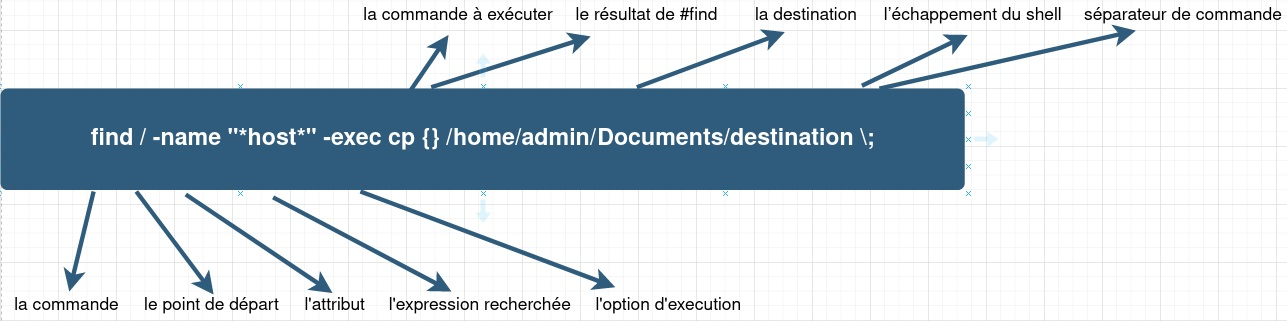
\includegraphics[scale=0.5]{Find.jpg}
			\end{flushleft}
	\chapter{Travailler avec des fichiers textes}
		\section{Comprendre VIM} 
			• Par tradition, il existe deux logiciels d’édition couramments utilisés pour réussir à éditer des fichiers en ligne de commande afin de ne pas devoir sortir du « SHELL »\\
			$\Rightarrow$ VIM (celui que nous allons voir)\\
			$\Rightarrow$ Emacs ( le plus compliqué des deux à maitriser)\\
			• Pour éditer un fichier texte avec « VIM » vous devez utiliser la commande vim [SOURCE DU FICHIER]\\
			• vim fonctionne sous 3 modes distinct :\\
			1) Le mode « command » : permet de sauvegarder, quitter, rechercher …\\
			2) Le mode « insert » : permet d’éditer le texte ...\\
			3) Le mode « visual » : permet d’effectuer des sélections dans le texte ...\\
			• Il est très important de comprendre que chaque action ne peut se faire que dans le mode qui lui est dédié
			• En fonction des modes « VIM » possède plusieurs options :\\
			- \underline{En mode COMMANDE :}\\
			- :w (sauvegarde votre fichier)\\
			- :q (quitte le fichier)\\
			- :! ( force l’action)\\
			- :wq ! (sauvegarde et quitte en forçant l’action)\\
			- u (undo)\\\\
			- \underline{En mode INSERT :}\\
			- Vous pouvez simplement l’utiliser comme un éditeur de texte sans l’option copier – coller.\\\\
			- \underline{En mode VISUAL :}\\
			- D (delete la sélection)\\
			- Y (copie la sélection)\\
			- P (colle la sélection)\\
		\section{Travailler avec le pager less} 
			• less [SOURCE] est une commande qui à la capacité d’organiser le texte en page pour le « SHELL ». \\
		\section{Lire un fichier texte grâce à cat et tac} 
			• Certain fichiers texte sont suffisamment court pour ne pas requérir à less.\\
		    • La commande cat [SOURCE] est alors utile pour présenter le contenu du fichier dans le « SHELL »\\
		\section{Lire le début ou la fin d’un fichier avec head tail} 
			• head -n[nombre de lignes] [SOURCE] : présente les 10 premières lignes du fichier dans le « SHELL »\\
		    • tail -n[nombre de lignes] [SOURCE] : présente les 10 dernières lignes du fichier dans le « SHELL »
		\section{Travailler avec la commande grep en dehors de |} 
			• grep est une des commandes les plus utiles en Linux.\\
		    • Exemple : vous chercher tout les fichiers ou il est écrit « dhcp » dans votre système.\\
		    • grep -iR [Expression recherchée] 2>/dev/null\\
		    • -i : attribut qui rend grep case insensitive\\
		    • -R : attribut qui permet à grep de travailler de manière récursive\\
		    • 2>/dev/null : redirection des erreurs dans le /dev/null\\
		\section{Comprendre les « REGEXP »} 
			• Les expressions régulière sont des modelé de texte utilisable	par des outils présent dans Linux comme grep\\
		    • Il ne faut pas confondre les « REGEXP » et le « globbing » Linux\\
			$\Rightarrow$ Le « globbing » est interne au « SHELL »\\
			$\Rightarrow$ Les « REGEXP » est générale et utilisable par toute les commandes qui traite des chaines de caractère.\\
			\begin{flushleft}
				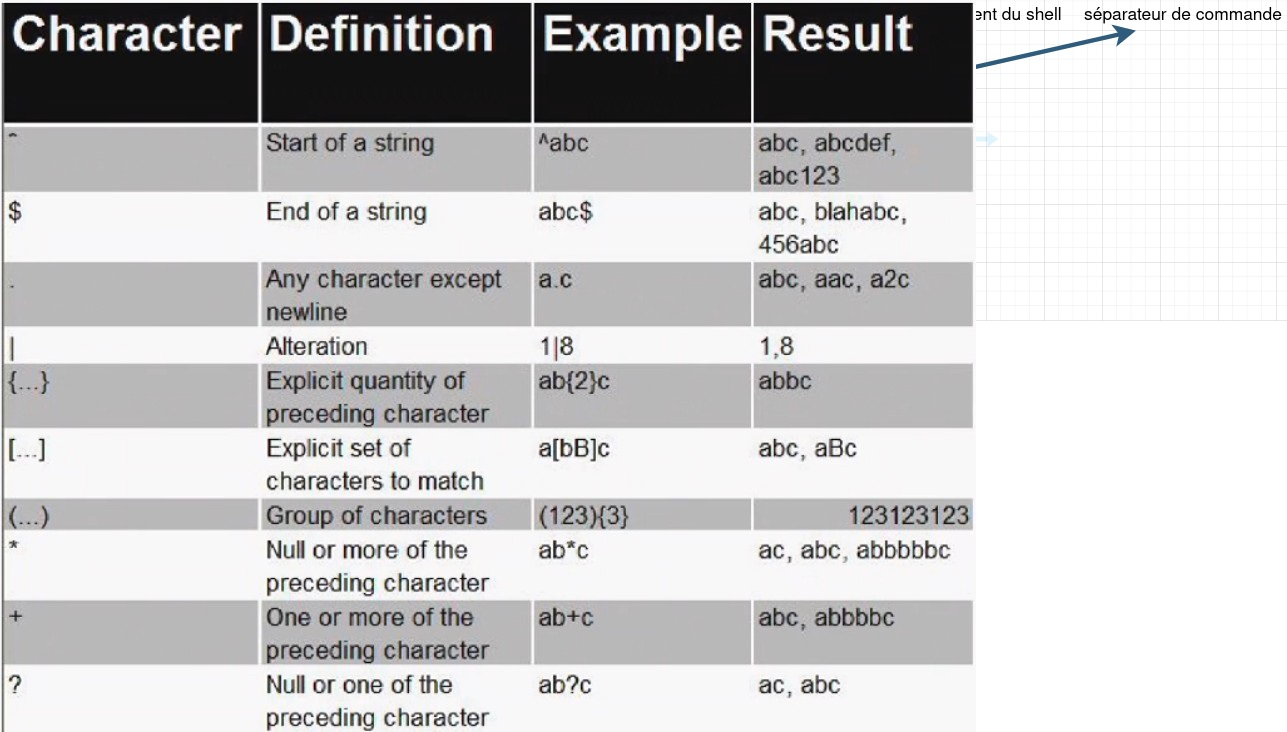
\includegraphics[scale=0.4]{REGEXP.jpg}
			\end{flushleft}
		\section{Utiliser les commandes awk, sort, tr} 
		    • awk est une commande qui permet de découper un texte en fonction de ses délimiteurs.
			\begin{flushleft}
				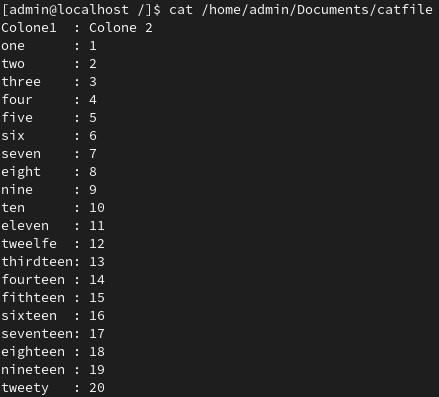
\includegraphics{AWK1.jpg}
			\end{flushleft}
			\begin{flushleft}
				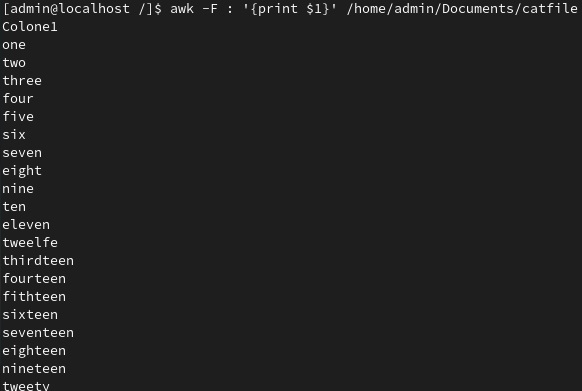
\includegraphics{AWK2.jpg}
			\end{flushleft}
			• sort est une commande qui permet de trier le texte dans l’ordre alphabétique ou numérique.\\
			$\Rightarrow$ sort [source] (alphabétique)\\
			$\Rightarrow$ sort -n [source] (numérique)\\
			• tr est une commande qui permet de réaliser une traduction de certains caractères du texte en d’autres\\
			$\Rightarrow$ tr [caractère(s) d’origine] [caractère(s) de remplacement]\\
			$\Rightarrow$ tr [état d’origine] [état de remplacement]
			\pagebreak 
	\chapter{Se connecter à un serveur}
		\section{Travailler en « root » ou en « local user »}
			•En Linux il existe deux types d'utilisateurs :\\
			$\rightarrow$ L'utilisateur normal appelé "local user"\\
			$\rightarrow$ Le super-utilisateur appelé "root"\\
			•Il est possible de se connecter en tant que "root" uniquement dans un "SHELL" précis et pas sur tout
			l’environnement grâce à la commande \color{red}sudo -i {\color{black}ou} grâce à sudo su -\\ 
			$\triangle$ 
			\textit{\color{black}
			Il faut éviter, tant que faire se peux, de travailler en "root"}\\
			\color{black}
		\section{Utiliser la commande su}
			•La commande {\color{red}su [LOGIN]} permet de se connecter à n'importe quel utilisateur (pour peu que l'on ai les droits d'administrations)\\
			•Pour effectuer des opérations admin il faut soit être le "root", soit faire partie des "sudoers" (=user capable de lancer la commande {\color{red}sudo})\\
			$\Rightarrow$ Pour cela, l'user doit faire partie du groupe "wheel"\\
			•{\color{red}id [USERNAME]} $\Rightarrow$ Montre l'UID, le GID, ainsi que les groupes auquels appartiennent l'user\\
			\pagebreak 	
		\section{Créer une configuration "sudo" simple}
			•Dans le système Linux, il existe un fichier qui régi les cas d’utilisation du sudo.\\
			{\color{red}visudo} $\Rightarrow$ Permet d'ouvrir ce fichier avec VIM et d'y effectuer des changements\\
		\section{Connexion à distance à un système Linux}
		    •\color{red}
			ssh [username]@[ip-address] {\color{black}ou} ssh [username]@[hostname] 
			\color{black}
			$\Rightarrow$ Permet de se connecter d'une machine Linux à une autre de manière sécurisée.\\
			\textit{Remarque : La commande {\color{red}telnet} existe également mais à tendance à disparaitre des nouvelles distri Linux car elle n'est pas sécurisée}
			\pagebreak 
	\chapter{La gestion des utilisateurs}
		\section{Importance des users} 
		    Users important car : \\
		   	•impossible de se connecter sans users. \\
			•Chaque processus appartient à un user. \\
			user accounts = personne physique ou entité système\\
			$\Rightarrow$ "Chaque fichier ou dossier DOIT posséder un user"
		\section{Création des users}
			•{\color{red}useradd [OPTIONS] [LOGIN]} $\Rightarrow$ Créer un user \\
			•{\color{red}useradd -g [GROUPE] [LOGIN] } $\Rightarrow$ Créer un user en lui attribuant un autre groupe primaire autre que lui-même (attention le groupe doit déjà exister)\\
			•{\color{red}useradd -G [GROUPES] [LOGIN]} $\Rightarrow$ Créer un « user » en lui attribuant des groupes secondaires  (attention les groupes doivent déjà exister)\\
			•Pour la gestion des paramètres de création par défaut des user voir {\color{blue}/etc/default/useradd}, {\color{blue}/etc/login.defs} et {\color{blue} /etc/skel/}
		\section{Suppression d'un user}
			•{\color{red}userdel [OPTIONS] [LOGIN]} $\Rightarrow$suppression d’un user
			\pagebreak 
		\section{Création groupes}
			•{\color{red}groupadd [OPTIONS] [GROUPE]} $\Rightarrow$ création groupe\\
			•{\color{red}usermod [OPTIONS] [LOGIN]} $\Rightarrow$ permet de modifier les paramètres d’un user déjà existant\\
			•{\color{red}usermod -g [NEW PRIMARY GROUP] [LOGIN]} $\Rightarrow$ change le groupe primaire du user\\
			•{\color{red}usermod -G [LIST OF SECONDARY GROUP] [LOGIN]} $\Rightarrow$ écrase la liste des groupes secondaires du « user » pour la remplacer par la nouvelle\\
			•{\color{red}usermod -aG [LIST OF SECONDARY GROUP] [LOGIN]} $\Rightarrow$ : ajoute sans écraser à la liste des groupes secondaires du user les nouveaux groupes
		\section{Modifications de groupes}
			•{\color{red}groupmod [OPTIONS] [GROUP]} $\Rightarrow$ Modifie un groupe déjà existant
		\section{Passwords}
			•\color{red}
			passwd [OPTIONS] login 
			{\color{black}OU}
			chage [OPTIONS] login
			\color{black}
			$\Rightarrow$ Permet d'ajouter ou supprimer des passwords\\
			•Le fichier {\color{blue}/etc/passwd} contient la liste des utilisateurs et est en accès non restreint.\\
			Il contient 7 champs : password : UID : GID : comment : homedir : shell\\
			•Le fichier {\color{blue}/etc/group} contient la définition des groupes et la liste des utilisateurs qui en font partie\\
			Il contient 4 champs : Group: password : GID : users ( tierce)\\
			•Le fichier {\color{blue}/etc/shadow} accompagne le fichier {\color{blue}/etc/passwd} et c’est là que sont stockés, entre autres, les passwords cryptés des utilisateurs ainsi que les informations relatives à leurs validités.\\
			•{\color{blue}/etc/gshadow} : C’est le pendant du fichier {\color{blue}/etc/shadow} mais pour les groupes. Il n’est cependant pas supporté dans certaines distributions LINUX anciennes\\
		Il contient 4 champs : Group : password crypté : admins du group : membres du groupe\\
			\textit{Remarque : La création des utilisateurs peut être entièrement effectuée à la main en travaillant sur les fichiers car se sont des fichiers plats (vivement déconseillé de le faire)}
	\chapter{Gérer les permissions et les quotas en Linux}
		\section{Les permissions en Linux} 
			• Le fonctionnement du système de permissions en linux est assez spécial de par son historique. Au début, personne ne pensait à la sécurité car on ne pensait pas au réseau. Lorsque les premiers développeur ont voulu apporter un semblant de sécurité, ils ont mit en place le système de permissions.\\
		    • Le système de permission se repose sur trois axes principaux :\\
		 	$\Rightarrow$ Les Users\\
		 	$\Rightarrow$ Les Groupes\\
		 	$\Rightarrow$ Les Autres \\
			• Les permissions se notent de deux manières différentes. Soit sous forme de lettres (U-User / G-Group / O-Others) soit sous forme de chiffre (sur base octale)\\
			\begin{flushleft}
				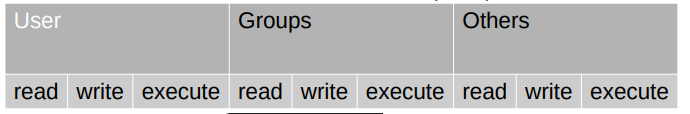
\includegraphics[scale=0.6]{PermissionsLettres.png}
			\end{flushleft}
			\begin{flushleft}
				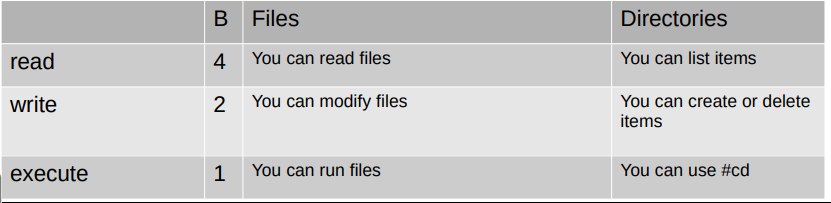
\includegraphics[scale=0.6]{PermissionsChiffres.png}
			\end{flushleft}
		 	1) Commande pour les permissions en UGO : chmod [UGO permissions] [PATH] \\
		 	2) Commande pour les permissions en Octal : chmod [octal permissions] [PATH] \\
			• UGO : « u » / « g » / « o » "+" ou "-" r-w-x pour ajouter/retirer un droit à un User \\
			• Octal : choix du chiffre octal en sachant que r=4, w=2, x=1. Il faut spécifier un chiffre octal pour chaque catégorie U-G-O (les droits ne s'ajoutent pas à ceux présent mais les écrasent) \\
			• il existe aussi des permissions spéciales pour gérer certain aspect non couverts par les permissions standards \\
			\begin{flushleft}
				\includegraphics[scale=0.6]{PermissionsSpéciales.png}
			\end{flushleft}
		 	1) Commande pour les permissions spéciales : chmod [UGO permissions] [PATH] (u+s pour les SUID, g+s pour les SGID et +t pour le stickybit) \\
			2) Commande pour les permissions spéciales en Octal : chmod [special permissions][octal permissions] [PATH] \\
		\section{Les ACL} 
			• Les permissions vue au dessus sont cependant pas suffisantes pour régler tout les problèmes qui arrivent c'est pourquoi les ACL (Access Control List) sont créés. \\
			• il existe deux sortes de ACL : les normales (appliquées sur les fichiers deja existants) et les default (fichier créés par la suite). la commande pour les gérer est : setfacl -Rm [Permissions Modification] [File/FOLDER PATH]. La seule différence va être la lettre utilisé après le Rm de la commande  (d pour default)  \\
			\begin{flushleft}
				
\includegraphics[scale=1]{ACL.png}
			\end{flushleft}
		    • Afin de vérifier les ACL d'un fichier on peut utiliser : getfacl [File/FOLDER PATH]\\
			• Les attributs éttendu ont été créé afin de pouvoir rejouter un couche de permissions sur les fichiers : il y a 2 commandes afin de les manipuler, lsattr pour les lister et chattr pour les modifier\\
		 	$\Rightarrow$ chattr +[ATTRIBUTS] [SOURCE] avec +/- pour ajout et retrait et -R pour l'appliqueer au reste des fichiers de cette branche.\\
		\section{Les Quotas}
			• Les quotas ont été inventé fin de restreindre des utilisateur pour ne pas qu'ils puissent saturer l'espace disque des serveurs. Il y a deux sortes de limites :   \\
			1) les quotas Softs qui sont des limites dépassable pendant un certain temps. \\
		 	2) les quotas Hard, qui ne permettent pas de dépassement. \\
			• Ces quotas peuvent s'appliquer sur deux types de limites : les inodes (le nombre de fichiers) et les blocks (la taille des fichiers).\\
			• la commande "quotaon" active les quotas ou "quotaoff" les désactive avec l'argument -a pour le faire sur tous. la commande "repquota -a" donne le statut actuel des quotas.\\
	\chapter{Configurer les éléments réseau}
		\section{Configuration réseau runtime}
			• En Linux, il existe deux types de configuration réseau : runtime (pour les test et le monitoring) et persistante (pour l'accès permanent au réseau).\\
			$\Rightarrow$ Pour travailler en runtime il faut utiliser la commande : ip [OPTIONS][OBJETS] !!! commande assez complète, l'utilisation de --help est conseillée. \\
			• La commande "ip link" permet de voir les interfaces réseau dispo et "ip address show" permet de les afficher avec leur adresse.\\
			$\Rightarrow$ "ip address show" : 1) Lo : interface  loopback, 2) enp... : interface physique, 3) WLP... : interface wireless, 4)Vibr0 : interface virtuelle pour machine virtuelle. \\
		  	1) ajout adresse ip sur interface : ip address add dev [INTERFACE NAME] [IP+mask] (on peut remplacer "add" par "del" ou "replace" pour en supprimer une ou la remplacer).\\
		 	2) ping interface : ping ip .\\
		 	3) default getaway : ip route show .\\
		\section{Configuration réseau persistante}
			• \textbf{nmcli}  : c'est le programme le plus performant et le plus courant pour faire des configuration réseau persistantes. Afin de naviguer fficacement dans nmcli il est très utile d'utiliser l'auto-completion du "bash". 2 options sont fort utilisées: Device et surtout Connection. \\
			1) "nmcli connection modify" afin de trouver la bonne interface à modifier. Il est donc possible assez facilement de s'y retrouver en utilisant l'auto-completion et en voyagant de proche en proche afin de pouvoir tout configurer.\\
			2) "nmcli connection up [CONNECTION NAME]" afin d'activer l'interface\\
			• /etc/hostname pour la modification du hostname \\
		    • /etc/hosts pour les hostname à distance\\
		    • /etc/resolv.conf nom et adresse ip des servurs dns !!! ne pas modifier sauf via nmcli\\
		    •/etc/nsswitch.conf pour les priorité dns\\ 
			$\Rightarrow$ ping [IP ADRESS / HOSTNAME] pour les test de connectivité à une interface \\
			$\Rightarrow$  dig [HOSTNAME] pur vérifier les dns et la validité du hostname\\
	\chapter{Liste des commandes Linux}
		\section{Commandes de bases sur le système de fichiers}
			\begin{tabular}{p{3cm}|p{11cm}}
		   		ls & Liste le contenu d’un répertoire\\
				cd	& Se déplace dans un répertoire\\
				cmp	& Comparer deux fichiers\\
				cp	& Copie un fichier ou répertoire\\
				locate & Rechercher des fichiers (peut ne pas être inclut par défaut)\\
				mv	& Déplacer/renommer un fichier ou répertoire\\
				rm	& Supprimer un fichier ou répertoire\\
				rmdir	& Supprimer un dossier\\
				mkdir	& Créer un dossier\\
				ln	& Créer un lien vers un fichier ou dossier\\
				lsof	& Lister les fichiers ouverts\\
				find	& Chercher un fichier dans l’arborescence\\
				file	& Indique le type de fichier\\
				rename	& Renommer un fichier selon un pattern\\
				which	& Renvoyer le chemin d’accès d’un fichier\\
				split	& Découper un fichier en plusieurs fichiers\\
				stat	& Renvoyer le statut d’un fichier (droits, attributs, propriétaire, …)\\
				touch	& Créer un fichier s’il n’existe pas ou change sa date d’accès s’il existe\\
			\end{tabular}
		\section{Commandes de bases sur les disques}
		    \begin{tabular}{p{3cm}|p{11cm}}
				blkid	& Imprimer les attributs du périphérique de bloc (partitions et support de stockage) comme uuid et le type de système de fichiers\\
				df	& Affiche l’espace disque et inobre libre\\
				du	& Affiche l’espace utilisé et donne l’occupation disque par dossier\\
				fsadm	& Utilitaire pour redimensionner ou vérifier le système de fichiers sur un périphérique\\
				fdisk	& Gèrer les disques et partitions de disque\\
				fsck	& Vérifier et réparer un système de fichiers Linux\\
				hwinfo	& hwinfo est un outil d’information matériel à usage général et peut être utilisé pour imprimer la liste des disques et des partitions\\
				lsblk	& Répertorier tous les blocs de stockage, y compris les partitions de disque et les lecteurs optiques\\
				mkfs	& Créer le système de fichiers (ex4, etc)\\
				mkfifo	& Créer des tubes nommés (FIFO) avec les NOM donnés\\
				parted	& Lister et modifier les partitions de disque\\
			\end{tabular}
    	\section{Commandes de bases sur les textes}
	        \begin{tabular}{p{3cm}|p{11cm}}
				awk / gawk	& Langage de balayage et de traitement des motifs\\
				cat	& Afficher le contenu d’un fichier\\
				cut	& Supprimer des sections d’un fichier\\
				grep	& Rechercher l’occurence dans un fichier\\
				head	& Afficher l’entête du fichier\\
				more	& Afficher le contenu d’un fichier page par page\\
				join	& Rejoint les lignes de deux fichiers partageant un champ commun de données.\\
				less	& Comme more mais en plus rapide\\
				look	& Montre les lignes commençant par un pattern\\
				nl	& Ecrit chaque fichier sur la sortie standard, avec des numéros de ligne ajoutés\\
				sed	& Recherche/remplacer, substitution de texte\\
				sort	& Trier le flux d’entrée\\
				tee	& Lit l’entrée standard et l’écrit à la fois dans la sortie standard et dans un ou plusieurs fichiers\\
				tail	& Affiche les dernières lignes d’un fichier\\
				tr	& Transforme une liste de caractère en une autre liste\\
				wc	& Afficher le nombre de lignes d’un fichier texte\\
			\end{tabular}   
		\section{Commandes de bases pour gérer les utilisateurs}
		    \begin{tabular}{p{4cm}|p{9cm}}
				adduser ou useradd	& Ajouter un utilisateur\\
				chmod	& Changer les droits sur un fichier ou dossier\\
				chown	& Changer le propriétaire\\
				chgrp	& Changer le groupe propriétaire\\
				deluser ou userdel	& Supprimer un utilisateur\\
				groups	& Renvoyer la liste des goupes dont l’utilisateur fait partie\\
				groupmod	& Modifier la configuration d’un groupe utilisateur\\
				id	& Renvoie les informationss UID – GID d’un utilisateur\\
				passwd	& Changer le mot de passe d’un utilisateur Linux\\
				su	& su (switch user) est une commande qui permet de s’identifier
				avec un autre utilisation ou passer une commande avec un autre utilisateur\\
				sudo	& Exécuter une commande avec un autre utilisateur\\
				users	& Montrer le nom d’utilisateur courant\\
				usermod	& Modifier un compte utilisateur\\
				who	& Affiche la liste des utilisateurs connectés à une machine (ordinateur)\\
		    \end{tabular}
	    \section{Le fonctionnement des utilisateurs et groupes sur Linux}
	        \begin{tabular}{p{3cm}|p{11cm}}
	    	    dmidecode	& Afficher les informations sytème par une extraction des structures de données SMBOIS\\
				free	& Afficher la mémoire utilisée et libre\\
				hdparm	& Récupérer des informations sur les disques\\
				hwinfo	& Afficher des informations très détaillées sur les périphériques d’un ordinateur\\
				lscpu	& Afficher les informations du processeur (CPU)\\
				lshw	& Afficher des informations très détaillées sur les périphériques d’un ordinateur\\
				lspci	& Répertorier tous les bus pci et les détails sur les périphériques qui y sont connectés.\\
				lsscsi	& Lister les périphériques SCSI\\
				lsusb	& Lister les périphériques USB\\
		    \end{tabular}
		\section{Commandes de bases sur les processus}
			\begin{tabular}{p{3cm}|p{11cm}}
		    	bg	& Passer un processus en tache de fond (background)\\
				fg	& Pour reprendre un processus arrêté en arrière plan\\
				kill	& Envoyer un signal à un processus pour le tuer\\
				nice	& Démarrer un processus avec une priorité définis\\
				renice	& Changer la priorité d’un processus\\
				pidof	& Donne le PID d’un processus\\
				ps	& Lister les processus\\
				top	& Afficher et classe les processus actifs (cpu – mém – temps)\\
		    \end{tabular}
		\section{Commandes de bases réseaux}
		    \begin{tabular}{p{3cm}|p{11cm}}
				arp	& Afficher et manipuler la table et cache ARP\\
				dig	& Effectuer des requêtes DNS très poussées (à installer)\\
				host	& Effectuer des résolutions DNS\\
				iftop	& Afficher l’utilisation réseaux par interface\\
				ip	& Lister les interfaces réseaux et afficher la configuration IP\\
				ifconfig	& Lister les interfaces réseaux et afficher la configuration IP\\
				iptraf	& Afficher l’utilisation réseaux par interface\\
				hostname	& Afficher et modifier le nom de la machine\\
				mtr	& Lancer un traceroute en continue et ainsi de visualiser sur quel noeud, les pertes se font.\\
				netstat	& Afficher les connexions établies, en attente, etc\\
				ngrep	& network packet analyzer – Analyser les paquets réseaux\\
				nmap	& Effectuer des scans de ports\\
				ping	& Ping sur un host\\
				route	& Afficher ou modifier les routes\\
				tcpdump	& Capturer et Analyser les paquets réseaux\\
				traceroute	& Effectuer un trace route sur un host\\
		    \end{tabular}
		\section{Les commandes réseau utiles de Linux}
		    \begin{tabular}{p{3cm}|p{11cm}}
				curl	& Commande de transfert HTTP\\
				scp	& Transfert de fichiers sécurisé via le protocole SSH\\
				rsync	& Créer un mirroir d’un dossier ou permet de synchroniser des dossiers\\
				wget	& Télécharger des fichiers depuis un serveur WEB\\
		    
		    \end{tabular}
		\section{tar, gzip, bzip, rar, ZIP, 7zip – La compression/décompression de fichiers sur Linux}
		    \begin{tabular}{p{3cm}|p{11cm}}
				alias et unalias	& Créer et supprimer un alias de commande\\
				date	& Afficher ou changer la date du système\\
				halt	& Ordonner l’arrêt du système\\
				echo	& Affiche un texte dans le terminal\\
				reboot	& Redémarrage/rebooter le PC\\
				sysctl	& Configurer les options du noyau Linux\\
				uname	& Afficher les informations du noyau Linux\\
				which	& Localiser une commande\\
				whereis	& Localiser un binaire\\
		   \end{tabular}
		   \backmatter
\end{document}
